\documentclass[10pt,a4paper]{article}
\usepackage[utf8]{inputenc}
\usepackage[T1]{fontenc}
\usepackage{lmodern}
\usepackage[margin=14mm]{geometry}
\usepackage{amsmath}
\usepackage{booktabs}
\usepackage{graphicx}
\usepackage{float}
\usepackage{array}
\usepackage{tabularx}
\usepackage{xcolor}
\usepackage{caption}
\usepackage{microtype}
\usepackage{hyperref}

\definecolor{navy}{HTML}{163A5F}
\definecolor{teal}{HTML}{218A80}
\definecolor{warningbg}{HTML}{FFF1E6}
\definecolor{warningline}{HTML}{C75B12}
\definecolor{lightblue}{HTML}{EAF3F8}
\hypersetup{colorlinks=true,linkcolor=navy,urlcolor=navy}
\captionsetup{font=footnotesize,labelfont={bf,color=navy},skip=2pt}
\setlength{\parindent}{0pt}
\setlength{\parskip}{2.4pt}
\setlength{\tabcolsep}{4pt}
\renewcommand{\arraystretch}{1.05}
\pagestyle{plain}
\sloppy

\newcommand{\compactsection}[1]{%
  \vspace{2pt}{\large\bfseries\color{navy}#1}\par\vspace{1pt}%
}

\begin{document}

\begin{center}
  {\LARGE\bfseries\color{navy} Synthetic-IMU UWB Fusion}\\[-1pt]
  {\large\bfseries Two-Page Performance Brief}\\[2pt]
  {\small Erlangen RotoArm replay, 28 May 2026 \quad $\vert$ \quad Zekai Xiao \quad $\vert$ \quad 10 July 2026}
\end{center}

\noindent\colorbox{warningbg}{%
  \parbox{\dimexpr\textwidth-2\fboxsep\relax}{%
    \textbf{\color{warningline}Synthetic-IMU declaration.}
    \textbf{All IMU data and all IMU performance values in this report are synthetic.}
    They were generated from the OptiTrack/Vicon-reconstructed tag trajectory and evaluated by offline replay; no physical IMU measurements were used, so the results are not hardware validation.
  }%
}

\compactsection{Study design}

The recorded UWB trajectories from 17 RotoArm captures (34 tag tracks) were replayed against optical ground truth. Synthetic 120~Hz accelerometer and gyroscope packets were generated at the reconstructed UWB antenna centre, after which each L-series model injected datasheet-informed noise, residual calibrated bias, random walk, timestamp jitter, quantisation, vibration sensitivity, and mounting error. For every sensor, five random seeds were evaluated across the A0/U4 production branch, UWB post-filters, IMU preprocessing variants, and PC-side fusion solvers. The primary metric is the five-seed mean of the track-level 3D P95 error; lower is better.

\compactsection{Overall fusion effect}

The pure-UWB B0 control reached 231.8~mm P95. The matched P4 UWB smoother reduced this to 138.9~mm, while the best synthetic-IMU rows reached 129.5~mm for the low-cost MPU6050-like L2 model, 114.9~mm for the ICM-45686 L16 model, and 112.1~mm for the industrial-reference Xsens L20 model (Table~\ref{tab:headline}). Thus L20 improved P95 by 119.7~mm (51.6\%) relative to B0 and by 26.8~mm (19.3\%) relative to the matched P4 UWB control.

\begin{table}[H]
\centering
\caption{Selected five-seed track-level results. ``P4 UWB'' isolates the gain due to adding synthetic IMU information after applying the same UWB-side smoother.}
\label{tab:headline}
\small
\begin{tabular}{@{}l l r r r@{}}
\toprule
Method & Best chain & P50 & P95 & RMSE \\
& & \multicolumn{3}{c}{[mm]} \\
\midrule
B0 pure UWB & A0/U4/P0/T1 & 105.8 & 231.8 & 132.8 \\
P4 UWB control & A0/U4/P4/T1 & 78.2 & 138.9 & 86.2 \\
L2 MPU6050-like & P4/I5/T4 & 75.0 & 129.5 & 83.4 \\
L16 ICM-45686 & P4/I5/T2 & 69.0 & 114.9 & 76.1 \\
L20 Xsens MTi-3 & P4/I5/T2 & 68.4 & 112.1 & 75.7 \\
\bottomrule
\end{tabular}
\end{table}

\begin{figure}[H]
\centering

\includegraphics[width=0.78\textwidth]{fig/phase4_spiky_track_xz_l2_l16_l20.png}\\[-1mm]

\includegraphics[width=0.78\textwidth]{fig/phase4_spiky_track_err3d_l2_l16_l20.png}
\caption{Fusion effect on the difficult R01/BS2DCE track. Top: optical truth (black), pure UWB (light blue), and three UWB+synthetic-IMU trajectories. Bottom: 3D error over time. Fusion removed all 178 in-plane jumps above 200~mm and reduced track P95 from 595.5~mm (B0) to 188.4, 183.3, and 166.6~mm for L2, L16, and L20, respectively.}
\label{fig:effect}
\end{figure}

\newpage

\compactsection{Twenty-way performance comparison}

The current registry contains 19 evaluated synthetic IMU scenarios. L6 and L9 are reserved identifiers without sensor definitions or results. To provide a complete 20-object comparison without inventing data, Figure~\ref{fig:twenty} and Table~\ref{tab:twenty} compare those 19 scenarios with the pure-UWB B0 control. Each IMU entry is the best five-seed A0/U4 production row selected independently for that sensor; this is a tuned upper-bound comparison, not a fixed-algorithm hardware ranking.

\begin{figure}[H]
\centering
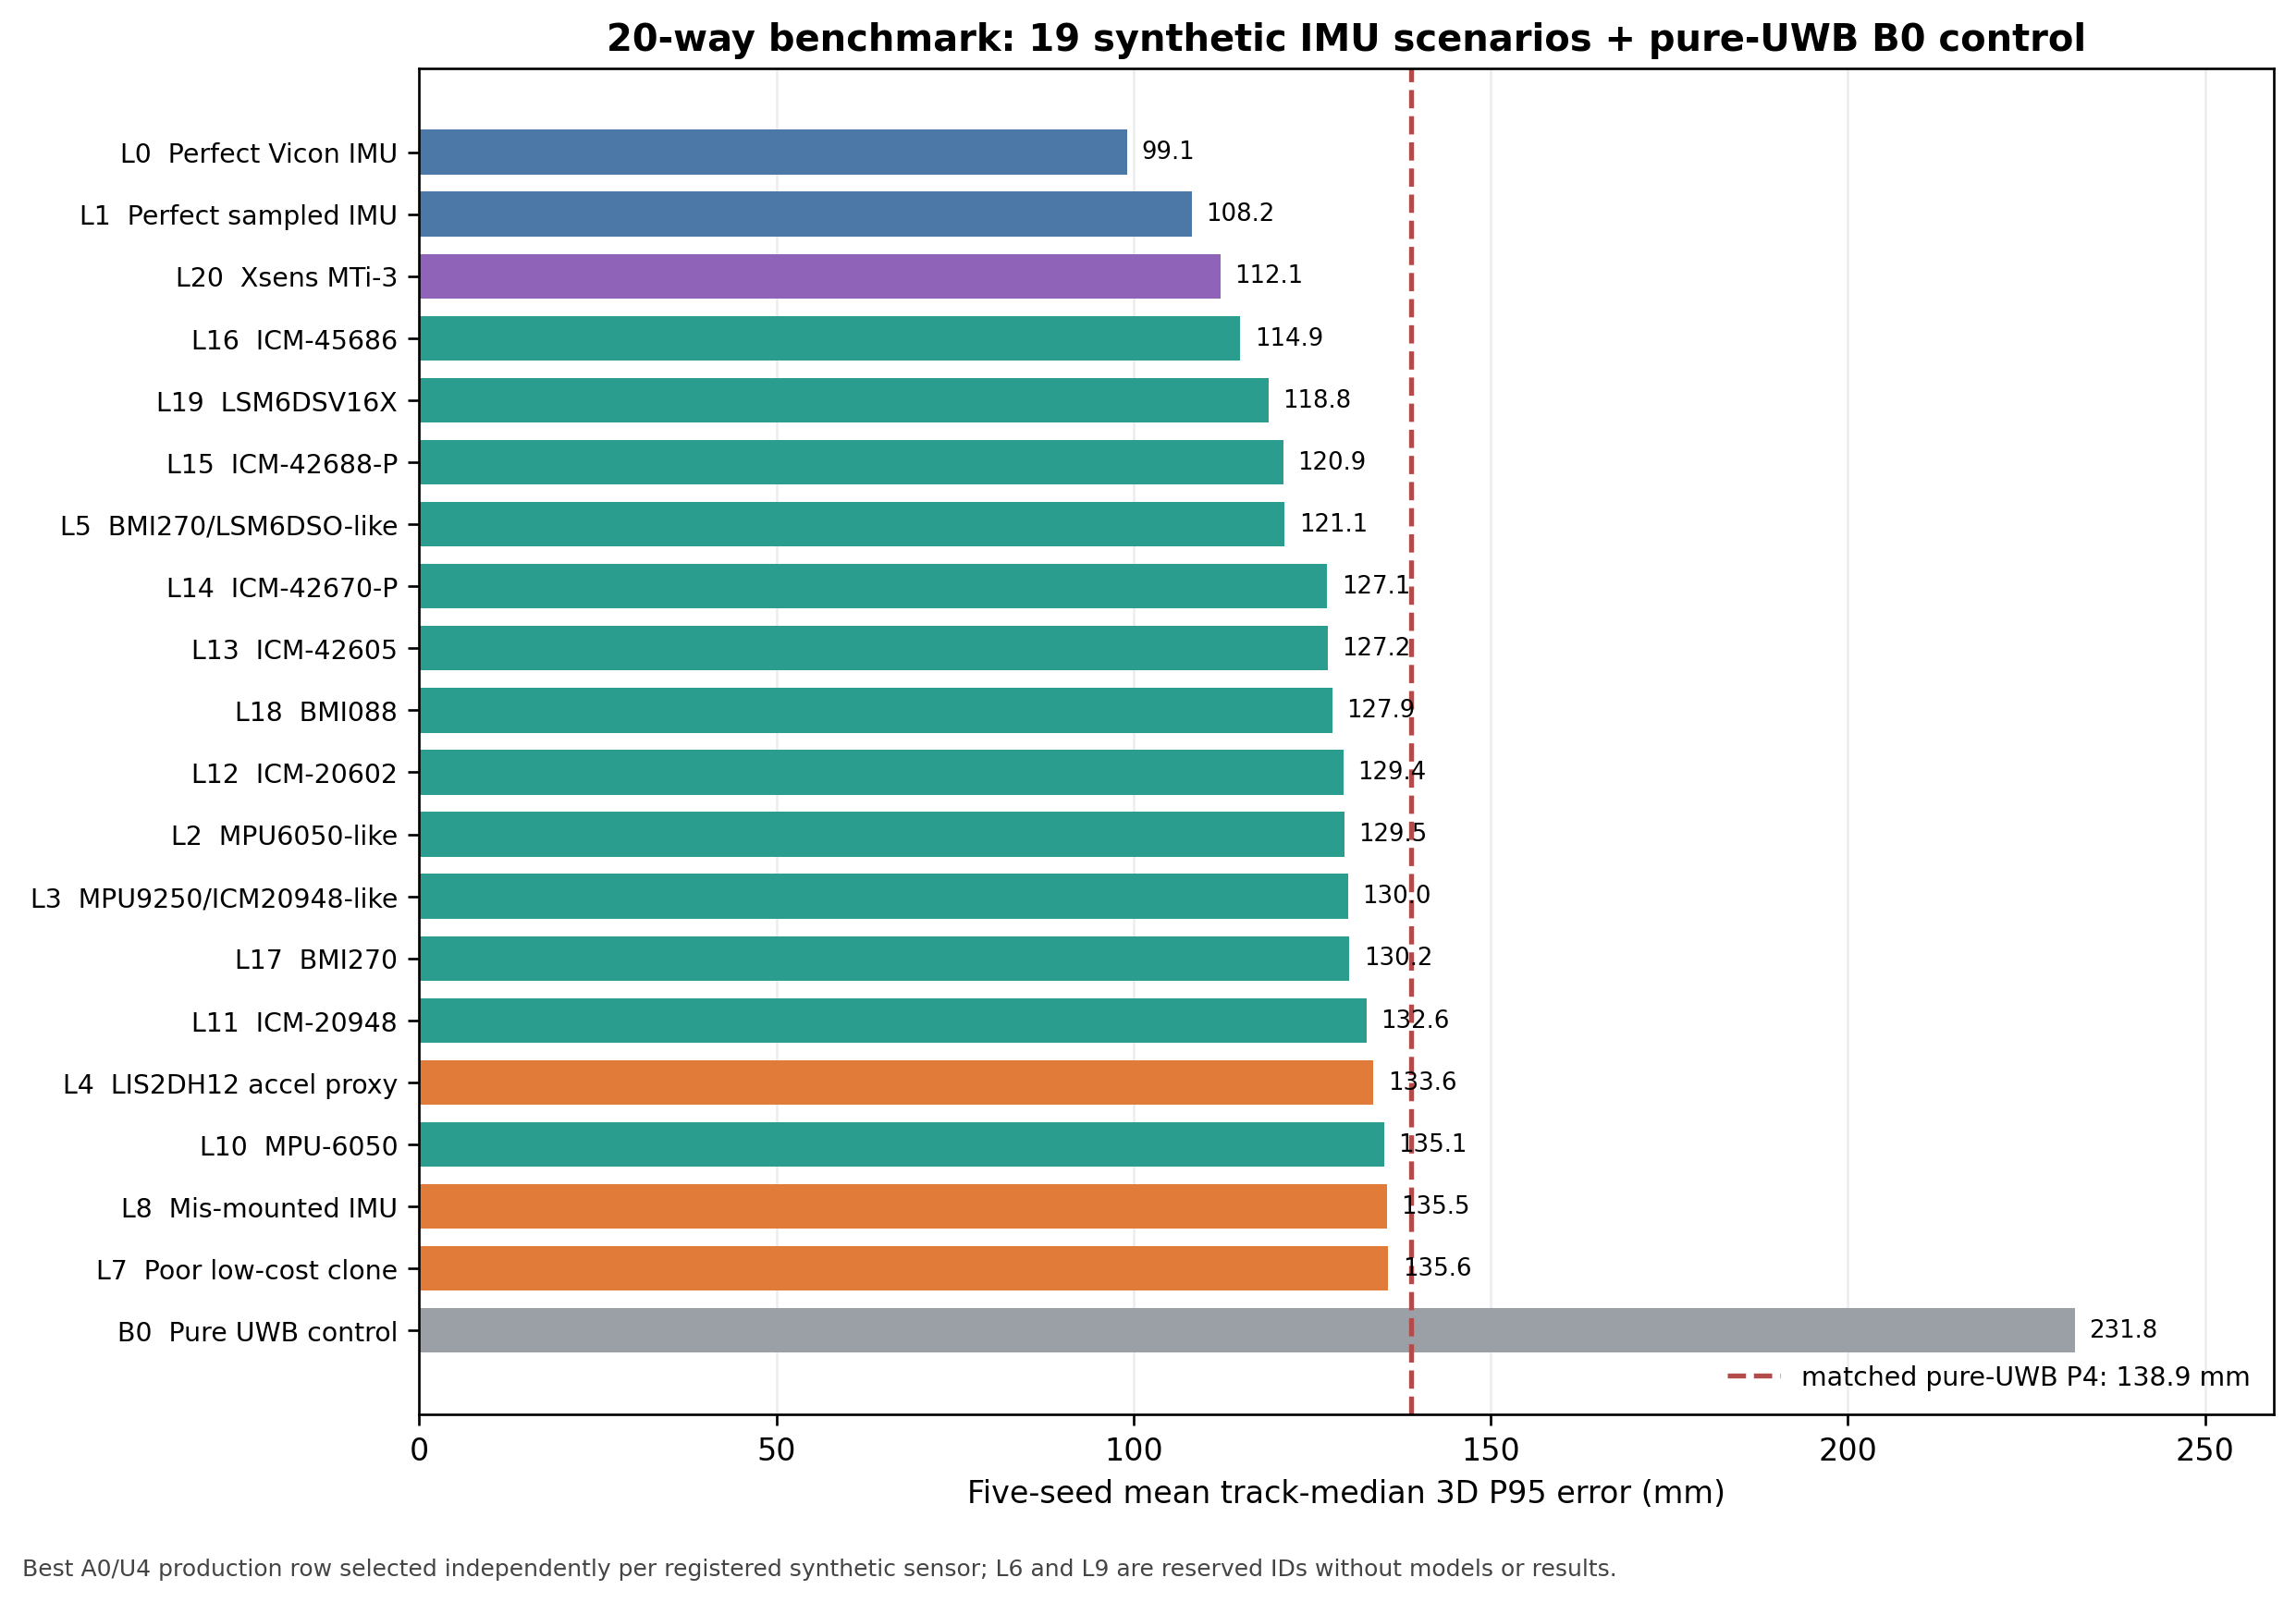
\includegraphics[width=0.73\textwidth]{fig/fusion_two_page_20way_performance.png}
\caption{Five-seed mean track-level 3D P95 for 19 registered synthetic IMU scenarios and the B0 pure-UWB control. The dashed line is the matched P4 pure-UWB result (138.9~mm). Blue denotes perfect diagnostic models, orange denotes negative-control or mounting-stress models, purple denotes the L20 industrial reference, and teal denotes the remaining sensor models.}
\label{fig:twenty}
\end{figure}

\begin{table}[H]
\centering
\caption{Numerical 20-way comparison. $\Delta$B0 is the P95 reduction relative to B0; positive values indicate improvement. L0/L1 are idealised diagnostics, while L4/L7/L8 are negative-control or stress scenarios.}
\label{tab:twenty}
\scriptsize
\begin{minipage}[t]{0.49\textwidth}
\centering
\begin{tabular}{@{}r l r r@{}}
\toprule
Rank & Scenario & P95 & $\Delta$B0 \\
& & \multicolumn{2}{c}{[mm]} \\
\midrule
1  & L0 Perfect Vicon & 99.1 & 132.7 \\
2  & L1 Perfect sampled & 108.2 & 123.6 \\
3  & L20 Xsens MTi-3 & 112.1 & 119.7 \\
4  & L16 ICM-45686 & 114.9 & 116.9 \\
5  & L19 LSM6DSV16X & 118.8 & 113.0 \\
6  & L15 ICM-42688-P & 120.9 & 110.9 \\
7  & L5 BMI270/LSM6DSO-like & 121.1 & 110.7 \\
8  & L14 ICM-42670-P & 127.1 & 104.7 \\
9  & L13 ICM-42605 & 127.2 & 104.6 \\
10 & L18 BMI088 & 127.9 & 104.0 \\
\bottomrule
\end{tabular}
\end{minipage}\hfill
\begin{minipage}[t]{0.49\textwidth}
\centering
\begin{tabular}{@{}r l r r@{}}
\toprule
Rank & Scenario & P95 & $\Delta$B0 \\
& & \multicolumn{2}{c}{[mm]} \\
\midrule
11 & L12 ICM-20602 & 129.4 & 102.4 \\
12 & L2 MPU6050-like & 129.5 & 102.3 \\
13 & L3 MPU9250/ICM20948-like & 130.0 & 101.8 \\
14 & L17 BMI270 & 130.2 & 101.6 \\
15 & L11 ICM-20948 & 132.6 & 99.2 \\
16 & L4 LIS2DH12 accel proxy & 133.6 & 98.2 \\
17 & L10 MPU-6050 & 135.1 & 96.7 \\
18 & L8 Mis-mounted IMU & 135.5 & 96.3 \\
19 & L7 Poor low-cost clone & 135.6 & 96.2 \\
20 & B0 Pure UWB & 231.8 & 0.0 \\
\bottomrule
\end{tabular}
\end{minipage}
\end{table}

\compactsection{Interpretation and limitations}

The dominant benefit is dynamic tail control rather than a large median shift: the synthetic inertial prior suppresses motion-inconsistent UWB excursions, while absolute UWB updates prevent unbounded inertial drift. L20 gives the best non-idealised P95, but L16 is only 2.8~mm worse and remains the strongest chip-class candidate in this replay. Even the low-cost L2 model improves on the matched P4 UWB control by 9.4~mm. The tightly coupled raw-range proxy is not selected because its best L20 row reached 465.4~mm P95, substantially worse than B0.

These results depend on the assumed sensor-error models, the circular RotoArm motion, offline access to the replay window, and independent tuning of the best chain for each sensor. They establish algorithmic potential under controlled synthetic perturbations, not real-time embedded performance. A defensible hardware claim requires time-synchronised physical IMU packets, calibration and mounting-error measurement, fixed-configuration testing on unseen motion, and latency/compute evaluation on the deployed tag pipeline.

\vfill
{\footnotesize\color{gray}Data provenance: \texttt{Analysis/IMU-Fusion-Simulation/runs/phase4\_algorithm\_factory}, five-seed TRUEFULL summaries; generated comparison data: \texttt{fusion\_two\_page\_20way\_performance.csv}.}

\end{document}
